\section{Introduction}

 % have been successful across a wide range of NLP tasks. %, paraphrase identification, sentiment analysis and relation extraction.  However, 
Existing computational models developed for natural language processing (NLP) tasks are vulnerable to dataset biases and spurious correlations in data, often referred to as ``shortcuts.''  % or annotation artifacts. 
These shortcuts enable models to achieve high performance on NLP datasets by exploiting surface-level correlations between features and labels. However, they also result in a significant performance drop on hard or slightly modified test data~\citep{naik-etal-2018-stress}. For example, in the area of natural language inference (NLI), models like BERT~\citep{devlin-etal-2019-bert} tend to misclassify premise-hypothesis pairs that contain ``negation'' words in their hypotheses as ``contradiction,'' which happen to be predictive features associated with the \textit{contradiction} label in certain NLI datasets~\citep{gururangan-etal-2018-annotation,poliak-etal-2018-hypothesis,modarressi-etal-2023-guide}.

% \hadi{related work, what has been done and what are the known findings. What's missing. cite all key papers.}

\begin{figure}[t]
    \centering
    \vspace{-20pt}
    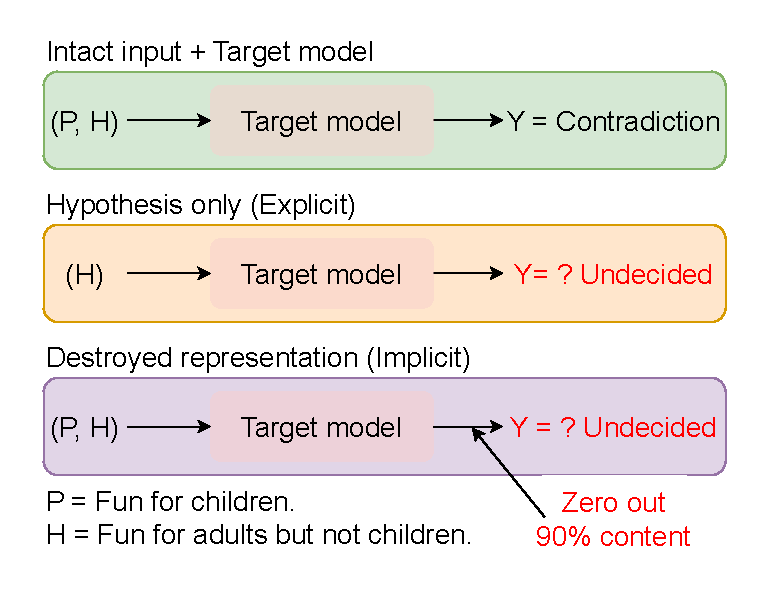
\includegraphics[width=.45\textwidth]{figure/motivating_example.pdf}
    % \vspace{-10pt}
    \caption{An example highlighting the concept of ``undecided learning'' using two types of data perturbation techniques. Given a premise-hypothesis pair in NLI, the model is expected to correctly classify their entailment relationship. However, given only the 
    % a grammatically perturbed 
    hypothesis, a robust model should be undecided, i.e., refrain from making a definite judgment 
    about the relationship between an unknown premise and %perturbed 
    the given hypothesis. Similarly, given a severely corrupted representation, a robust model should be undecided about the relation between a corrupted premise and hypothesis pair.
    Models that retain confidence in assigning labels to such inputs are likely to rely on shortcuts. \OursName takes an undecided stance against such inputs.}
    \label{fig:motivating_example}
    \vspace{-10pt}
    \label{fig:example}
\end{figure}

Existing debiasing approaches %employ external models to 
can detect known~\citep{clark-etal-2019-dont,sanh2020learning,karimi-mahabadi-etal-2020-end,modarressi-etal-2023-guide} and previously unidentified or unknown~\citep{utama-etal-2020-towards,sanh2020learning} biases in training data.
They mitigate dataset biases by 
re-weighting examples~\citep{sanh2020learning,karimi-mahabadi-etal-2020-end}, 
learning robust representations~\citep{gao-etal-2022-kernel,du-etal-2023-towards}, 
learning robust feature interaction patterns~\citep{wang-etal-2023-robust}, or 
reducing the effect of biased model components~\citep{meissner-etal-2022-debiasing}.

% Comments
% Existing
% (the original model)
% (external representations) 
% (parts)
% Any other approaches?

% \hadi{the need to investigate the missing parts. and how you do that.}s
% There are several key challenges that may compromise the effectiveness of existing approaches in mitigating dataset biases. 
Despite the significant progress made in addressing dataset biases, existing models have certain limitations:
\textbf{(a)}: they often adopt a {\em single view} to dataset biases and primarily focus on specific types of biases~\citep{clark-etal-2019-dont,karimi-mahabadi-etal-2020-end}. However, rich sources and diverse types of dataset biases can be present in the data.
\textbf{(b)}: existing approaches that are based on weak learners~\citep{utama-etal-2020-towards,sanh2020learning,ghaddar-etal-2021-end,meissner-etal-2022-debiasing} rely on a {\em single} weak learner to identify biases, which inevitably tie their performance to the capabilities of the chosen weak learner.
\textbf{(c)}: prior works often evaluate debiasing methods using BERT-based models, which may limit their generalizability to other model architectures. 

% which largely bounds these approaches by the learning capability of the weak learner.
% to insufficient regularization of model parameters against biased examples or cascade biases throughout the multi-stage training process. 
%debiasing
% Finally, existing methods are often tailored to specific NLP tasks due to the reliance on task-specific model architectures, which can restrict the transferability of the methods to different domains or problem settings. For example, Debias Mask~\citep{} does not work for embedding models, such as TransE~\citep{}. 
% We want to attend to bias when needed. 

% \hadi{2--3 key,contributions.}
We tackle the above challenges by developing \OursName--a multiview contrastive learning framework that mitigates dataset biases by being {\em undecided} in its prediction for biased views of data samples (see \textbf{Figure~\ref{fig:example}}). Specifically, the proposed method employs several data perturbation operators to generate biased views of intact data samples and integrate them into the training data and learning process. 
When presented with biased inputs, the model is trained to be undecided about the possible labels by making a uniform prediction across the label set. At the same time, the model is encouraged to be confident about intact inputs, which {\em often} serve as a reference for unbiased samples. Therefore, the approach encourages learning representations that are more attentive to the true signal of the underlying tasks rather than relying on shortcuts that are specific to certain datasets. 
In addition, the inherent randomness of the implicit perturbations in FairFlow (\S\ref{sec:imp_bias}) exposes the model to a diverse range of perturbations and prevents it from overfitting to specific types of biases present in the data.\looseness-1

The contributions of this paper are: 
\begin{itemize}
    \itemsep-1pt 
    % \itemindent-10
    \item categorization of dataset biases: we categorize prevalent data biases in NLU and model them using data perturbation operations;
    
    \item bias mitigation as an ``undecided learning'' problem: we formulate the bias mitigation problem as an ``undecided learning'' problem, which encourages reliance on genuine and task-related signals for effective debiasing;  
    % the approach can be applied to existing debiasing strategies in prior research. 
    %Specifically, in the presence of biased inputs, our approach ensures that the model's predictions are uniform across the label set, while it remains confident in predicting the labels of intact--mainly unbiased--data samples.
    \item robust performance on challengng samples: our approach shows robust results on {\em harder} test data while maintaining strong in-domain performance across several NLU tasks.\looseness-1
    % \item Our framework employs the Attention mechanism and can learn when to attend to bias and when not to. It also serves as an interpretability tool to recognize and classify spurious data.
    % \item Our framework is flexible to work with many debiasing strategies, including Product of Experts (PoE), Focal Loss (FL), etc.
    % \item We conduct extensive experiments on various types of NLP tasks, uncovering the disadvantages existing debias methods.
\end{itemize}

The experimental results show that \OursName obtains substantial improvement over competing models. Specifically, it achieves an average performance gain of 10.2 points on stress test datasets across several NLU tasks while maintaining performance on the original test sets. In addition, models trained using our framework show strong transferability, resulting in an average gain of 3.7 points in transfer testing experiments across different datasets and domains. 
Furthermore, 
% Our findings shed light on the biases present in existing debiasing methods, which still leave room for enhancement. Specifically, 
we show that existing methods can be further improved by incorporating the proposed perturbation operators within their original objectives, resulting in a substantial average improvement of 5.8 points on stress test sets across datasets. 
% with Product of Experts~\citep{10.1162/089976602760128018}. 
% In addition, we illustrate that existing debiasing methods still rely on shortcuts.


